\documentclass[report]{iisthesis}
%           or master (bachelor or master is required)

% These two packages are highly recommended:
\usepackage[T1]{fontenc} % make non-ASCII characters cut&pastable in PDF
\usepackage{lmodern}     % easiest way to get outline fonts with T1 encoding

% \usepackage[ngerman]{babel}     % if the thesis is written in German

\title{Rotating Table Task with Reconfigurable Behavior Trees}
\author{Fabian Amhof \\ Matteo Quaratino}
\supervisor{Dr. Matteo Saveriano}
%\supervisor{Firstname1 Lastname1\\ Firstname2 Lastname2}


\begin{document}
\maketitle
\tableofcontents
\label{chap:declare}

\chapter{Introduction}
In this project we have a rotating table with an Object on it. The task is to grab this object with a "Franka Emika Panda Robot", pick it up, and then place it again on the table. It was provided some work from last years course, where the basic functionality is already implemented. So the robot already grabs already the object and places it again on the table but he does it in a way that can be improved in many terms.
This implementation does not estimate the table velocity, they only have hardcoded some static offset to the objects position. Because of that the robot failed some times when he tried to grab the cube. 

\chapter{Improvements}
\label{improvements}

\section{Control Robot by ROS-node on external machine}
\label{separate_node}
We propose to control the robot with a ROS-node on a external machine. 
We think that it is more flexible, so you can easily change the ROS-node to reconfigure the robots behaviour without changing the scripts on the robot itself. In addition to that an external node allows we can write full-fledged software and not just
some scripts, expecially in regard to the RBT it's beneficial

\section{Estimate Table Velocity}
\label{estimate_velocity}
In the example we were given the robot arm does not adjust its movement in relation to the speed at which the table 
turns. The timing and movement speed is hardcoded, and so is the speed of the table. \\
We want to work on this by letting the arm adjust its movement dynamically to the table speed.

\section{Improve Grabbing Capabillities}
\label{improve_grabbing}
The grabbing motion of the current implementation is reliant on the table turn speed being a specific and constant value, since it's hardcoded. If it varies even by the slightest bit
the arm could potenionally run into problems and for example push the cube off the table, ideally this should not happen at all. \\
We want it to react accordingly by building on \ref{estimate_velocity}, assuming that a faster cube is harder to grasp, it might be necessary to define another grabbing motion 
or at least change it for different situations, like a uneven speed of the table. \\
In the given implementation the gripper does not rotate according to the alignment of the cube. The robot is not using joint number 7, which is responsible for the rotation of the gripper, we would like to try to allow the arm to adjust the angle of the gripper accordingly.
If all goes well, a option to reposition a misaligned cube could also be implemented.

\section{Implement RBT}
\label{implement_rbt}
That highlevel desicion making, for example if the robot should move its arm or try to grab something, can be done with behaviour trees or reconfigurable behaviour trees.
Reconfigurable behaviour trees are an extention of standard behaviour trees and provide a more dynamic and resource-saving approach to represent a task.
We will use RBT to plan the actions the robot should make in order to execute the task successfully. RBTs can execute different BT based on the priority of each subtask. The priority gets influenced by sensory data or states.
Based on the following parameters we would like to change priority of the different subtasks. Each subtask is represented in its own BT.
\begin{center}
    \begin{tabular}{ |c|c||c|  }
        \hline
        Object in reach & Object grabbed & Priorized Task \\
        \hline
        \hline
        False & False & Wait \\
        False & True & *Not possible* \\
        True & False & Grab Object \\ 
        True & True & Place Object on Table \\
        \hline
    \end{tabular}
\end{center}
\noindent
Since this is a relatively easy task it would be also easy to represent it with a normal BT. However when we use a RBT the table above would be a way how to deal with priorities. Another way is to just consider the distance of the object in the priority function and use the parameter "object grabbed" as precondition for the task "Place Object on Table".
Therefore if the object is not in reach the robots executes the "wait" task and when the object is in reach the instanciator first checks if the condition "object grabbed" is set. If it is set, then "Place Object on Table" gets executed, if not then "Grab Object" gets executed.

%\section{Use Camera to detect Cube [OPTIONAL]}
%\label{use_camera}
%Another thing that could be improved is the recognition of the object. At the moment, thanks to the simulation, we know the position of the object and so we dont have to recognize it. In the real world however we need some sensor to determinate the position and orientation of the object that we need to pick up. For this one could use a camera and then, based on the position of the camera and the image check where the object lies on the table. \\
%We would like to focus on the previous points and add this feature only when we're satisfied with section \ref{separate_node} to \ref{implement_rbt}. 

\chapter{Starting point}
This report builds on a previous work where a 'Franka Emika Panda Robot' grabs a object from a rotating table and replaces it.
The previous implementation had inverse kinematics already in place which we decided to keep. Furthermore all the code was done in LUA scripts, directly in CoppeliaSim which had to be moved to a external ROS-node to facilitate the addition of the reconfigurable behaviour tree.
Many parameters such as the time the arm takes to reach a position and the offset, that is needed to 'catch' the object in time, were hardcoded. This poses a problem when the speed of the rotating table changes and weill be calculated dynamically in our implementation.

\begin{figure}[h]
    \caption{Franka Robot in CoppeliaSim}
    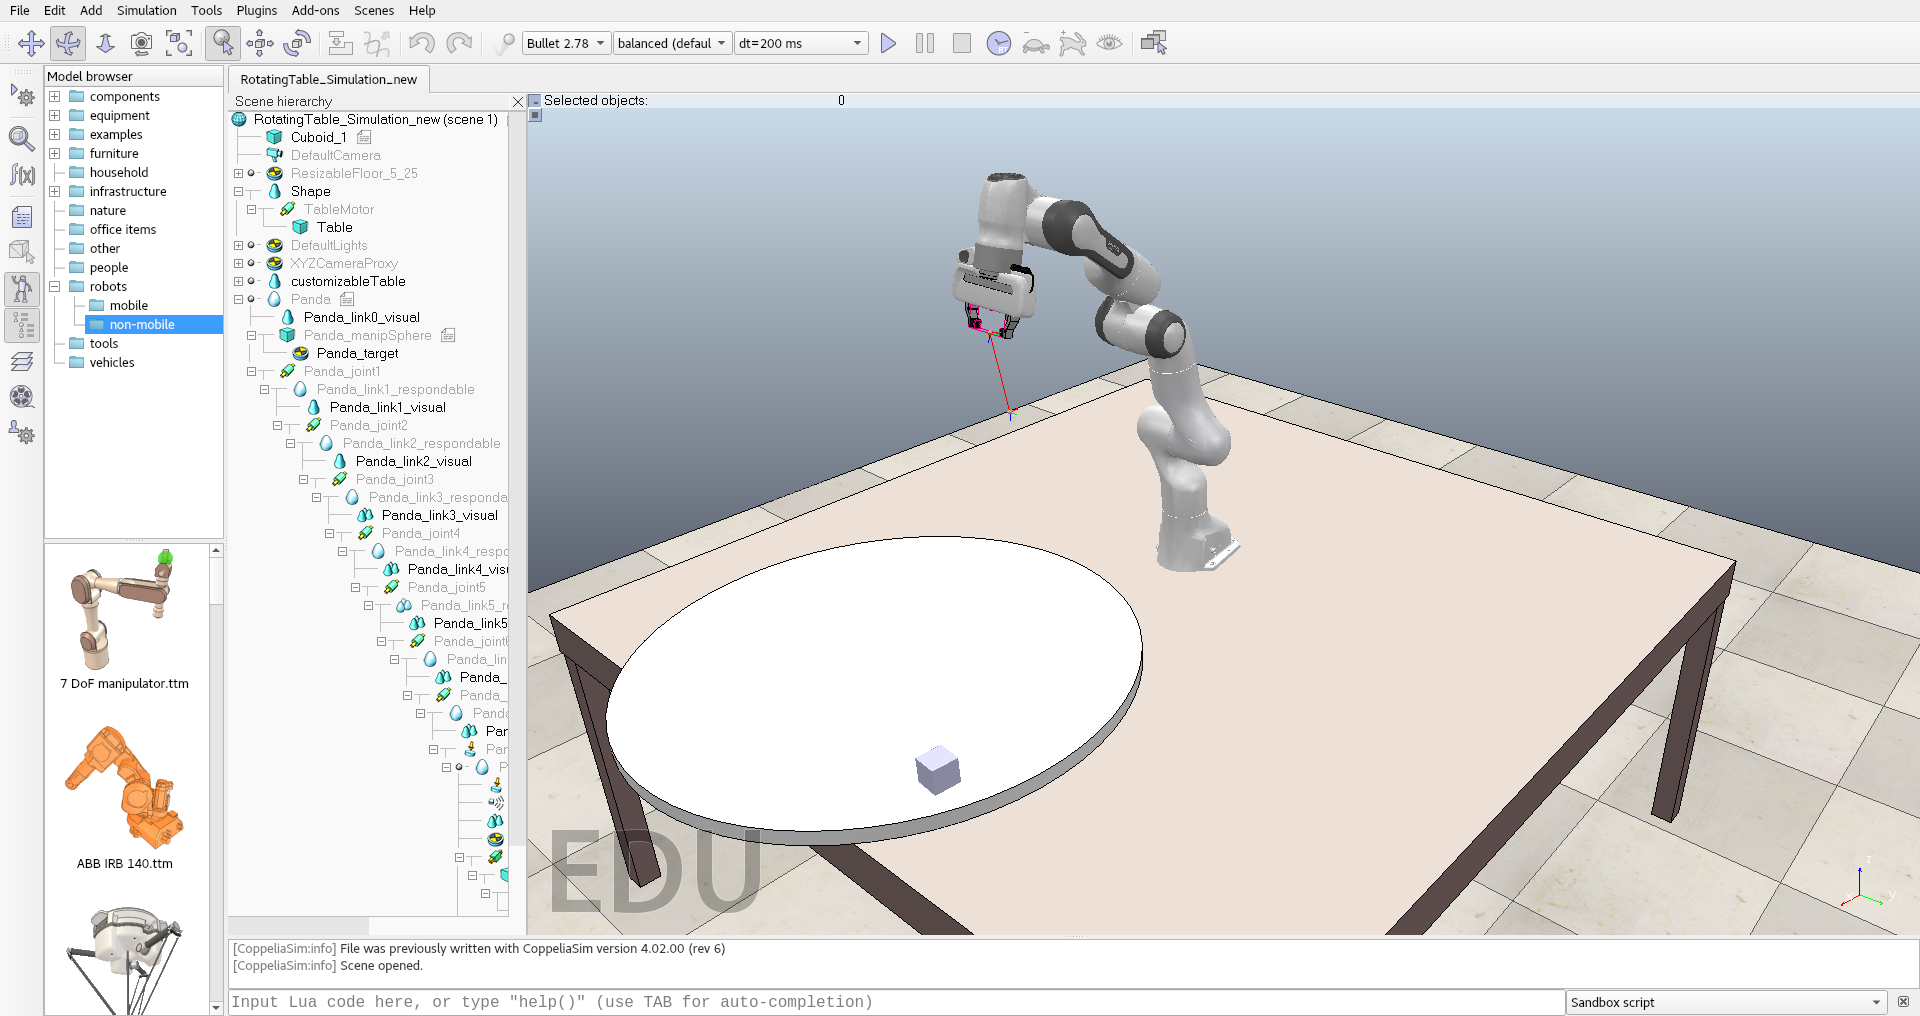
\includegraphics[width=\textwidth]{arm_coppeliaSim}
\end{figure}

\chapter{Implementations}
Here we document the realisazion of the suggested improvements.
\section{External ROS-node}
The first thing that had to be done was to allow the robot to interface with a python program.
This was important since the code for reconfigurable behaviour trees was implemented in python, so it would be easiest way to control the 
arm.
We created a few ROS-topics that would be useful:

\begin{description}
    \item [cube\_ori] the orientation of the cube in euler coordinates 
    \item [cube\_pos] the position of the cube in relation to the robot arm
    \item [gripper\_pos] the position of the gripper which will grab the cube
    \item [gripper\_state] controls the actuation of the gripper
    \item [robot\_state] integer which determines the state in which the robot is 
    \item [target\_pos] the position to which the gripper will move
\end{description}
\noindent
Firstly we moved the whole control of the arm from the LUA-script to a external python program, keeping only the inverse kinematics.
After this we could start to work on our suggested improvements. 

\section{Reconfigurable Behavior Trees}
Next the RBT \cite{DBLP:journals/corr/abs-2007-10663}, which was written in python was added. \\
This allowes to create trees in .json, which control the the arm, instead of using the automata-like system
from before.
Building on the code given to us we can program the necessary steps which will then bes used by the tree when controlling the arm, e.g. prediction of
the future position of the cube and its orientation.

\section{Determine table velocity and predicted position}
By measuring the position two times with a delay inbetween, we can calculate the rotational speed of the object and predict its position after a given peiod.
In order for the predicted position to be accurate the arms movement velocity and its distance from the cube has to be estimated aswell.
The last point is quite problematic, since 

\chapter{Reusability and Applicability}
The implementation we provide can be reused and repurposed easily since it is based on reconfigurable behaviour trees. The reconfigurable behaviour trees allow to alter the arms functionality
by adding actionnodes or altering them. This makes it more customizable than the version which was given to us. \\
If the project was to be ported to a physical version some adjustments have to be made:
\begin{description}
    \item[Object position] The arm gets its target position from the RBT via ROS-topics, it is calculated with the cube position, which in turn is also a ROS-topic. In order for a physical arm to know where to move, a sensor or camera needs to be put in place instead. 
    \item[] 
\end{description} 


\bibliography{refs}
\end{document}
